% Fig. 2 of the ICPC paper: one circuit, the slices of each dependence rule, and the dependence edges
% the rules build. Every slice and verdict was computed by the study's code (experiments/: slicers in
% slicers/registry.py, ground truth icpc/influence.py, oracle icpc/oracle_icpc.py) on this circuit:
%   ry(0.9) q2; x q1; h q1; h q0; cx q0,q1; h q0; cx q1,q2; z q1
% criterion q0: Dep {1..5}; DU {3,5} F=0; QPDG {0..5}; wire {1..5}
% criterion q2: Dep {0,1,2,3,4,6}; wire = Dep; QSlice at |000> {0,2,6}, F=1 at |000>, unsound at 20/20 Haar inputs
\documentclass[tikz,border=2pt]{standalone}
\usepackage{amsmath,amssymb}
\providecommand{\ket}[1]{\lvert #1\rangle}
\usetikzlibrary{arrows.meta,positioning,calc,backgrounds}
\definecolor{cblue}{HTML}{0072B2}
\definecolor{cver}{HTML}{D55E00}
\definecolor{cora}{HTML}{E69F00}
\definecolor{cgreen}{HTML}{009E73}
\definecolor{cgrey}{HTML}{8C8C8C}
\begin{document}
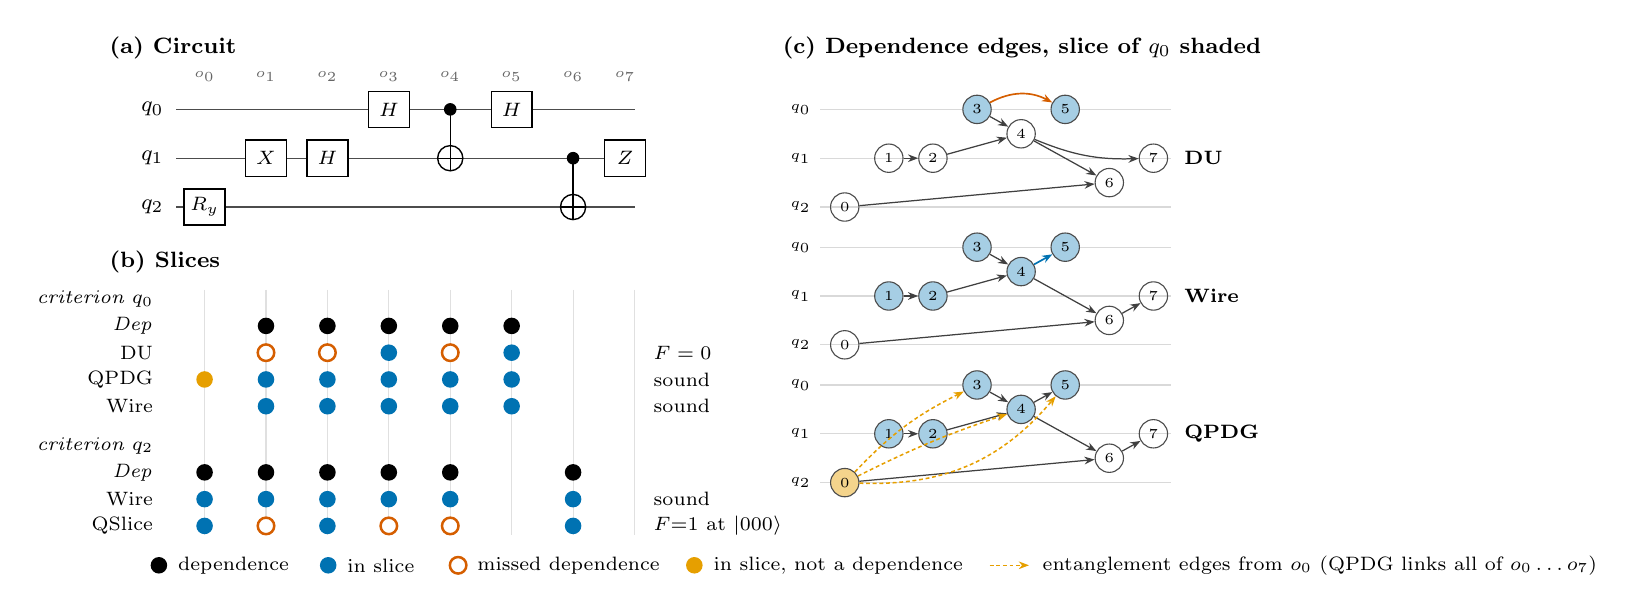
\begin{tikzpicture}[
  font=\footnotesize,
  wire/.style={draw=black!70, line width=0.5pt},
  gate/.style={draw=black, fill=white, line width=0.5pt, minimum width=5.2mm, minimum height=4.6mm, inner sep=0pt, font=\scriptsize},
  ctrl/.style={circle, fill=black, inner sep=0pt, minimum size=1.6mm},
  targ/.style={circle, draw=black, fill=white, line width=0.5pt, inner sep=0pt, minimum size=3.2mm, path picture={\draw[line width=0.5pt] (path picture bounding box.north) -- (path picture bounding box.south) (path picture bounding box.west) -- (path picture bounding box.east);}},
  idx/.style={font=\tiny\itshape, text=black!60},
  dot/.style={circle, inner sep=0pt, minimum size=2.1mm},
  insl/.style={dot, fill=cblue},
  spur/.style={dot, fill=cora},
  miss/.style={dot, draw=cver, line width=0.9pt, fill=white},
  dep/.style={dot, fill=black},
  gnode/.style={circle, draw=black!70, line width=0.4pt, minimum size=3.6mm, inner sep=0pt, font=\tiny},
  sl/.style={gnode, fill=cblue!35},
  dedge/.style={-{Stealth[length=1.3mm]}, line width=0.45pt, draw=black!75},
  eedge/.style={-{Stealth[length=1.3mm]}, line width=0.55pt, draw=cora, dash pattern=on 1.4pt off 1pt},
]
\def\dx{0.78}  % column spacing
\def\dy{0.62}  % wire spacing
% ------------------------------------------------------------------ (a) circuit
\begin{scope}
  \foreach \q/\y in {0/2,1/1,2/0} {
    \draw[wire] (0.42,\y*\dy) -- (8.0*\dx,\y*\dy);
    \node[anchor=east] at (0.38,\y*\dy) {$q_{\q}$};
  }
  % o0 RY q2
  \node[gate] at (1*\dx,0*\dy) {$R_y$};
  % o1 X q1, o2 H q1
  \node[gate] at (2*\dx,1*\dy) {$X$};
  \node[gate] at (3*\dx,1*\dy) {$H$};
  % o3 H q0
  \node[gate] at (4*\dx,2*\dy) {$H$};
  % o4 CX q0 -> q1
  \draw[line width=0.5pt] (5*\dx,2*\dy) -- (5*\dx,1*\dy);
  \node[ctrl] at (5*\dx,2*\dy) {};
  \node[targ] at (5*\dx,1*\dy) {};
  % o5 H q0
  \node[gate] at (6*\dx,2*\dy) {$H$};
  % o6 CX q1 -> q2
  \draw[line width=0.5pt] (7*\dx,1*\dy) -- (7*\dx,0*\dy);
  \node[ctrl] at (7*\dx,1*\dy) {};
  \node[targ] at (7*\dx,0*\dy) {};
  % o7 Z q1
  \node[gate] at (8*\dx-0.12,1*\dy) {$Z$};
  % operation indices
  \foreach \k in {0,...,7} { \node[idx] at ({(\k+1)*\dx - (\k==7?0.12:0)}, 2*\dy+0.42) {$o_{\k}$}; }
  \node[anchor=west, font=\footnotesize\bfseries] at (-0.55,2*\dy+0.78) {(a) Circuit};
\end{scope}
% ------------------------------------------------------------------ (b) slice matrix
\begin{scope}[yshift=-0.75cm]
  \node[anchor=west, font=\footnotesize\bfseries] at (-0.55,0.05) {(b) Slices};
  \def\rowA{-0.42}
  % row labels and rows: criterion q0
  \node[anchor=east, font=\scriptsize\itshape] at (0.25,\rowA+0.0) {criterion $q_0$};
  \foreach \lab/\r in {$\mathit{Dep}$/1, DU/2, QPDG/3, Wire/4} {
    \node[anchor=east, font=\scriptsize] at (0.25,\rowA-\r*0.34) {\lab};
  }
  % Dep q0 = {1,2,3,4,5}
  \foreach \k in {1,2,3,4,5} { \node[dep] at ({(\k+1)*\dx - (\k==7?0.12:0)},\rowA-1*0.34) {}; }
  % DU q0 = {3,5}; missed 1,2,4
  \foreach \k in {3,5} { \node[insl] at ({(\k+1)*\dx},\rowA-2*0.34) {}; }
  \foreach \k in {1,2,4} { \node[miss] at ({(\k+1)*\dx},\rowA-2*0.34) {}; }
  % QPDG q0 = {0..5}; spurious 0
  \foreach \k in {1,2,3,4,5} { \node[insl] at ({(\k+1)*\dx},\rowA-3*0.34) {}; }
  \node[spur] at (1*\dx,\rowA-3*0.34) {};
  % Wire q0 = {1..5}
  \foreach \k in {1,2,3,4,5} { \node[insl] at ({(\k+1)*\dx},\rowA-4*0.34) {}; }
  % verdicts
  \node[anchor=west, font=\scriptsize] at (8.0*\dx+0.12,\rowA-2*0.34) {$F=0$};
  \node[anchor=west, font=\scriptsize] at (8.0*\dx+0.12,\rowA-3*0.34) {sound};
  \node[anchor=west, font=\scriptsize] at (8.0*\dx+0.12,\rowA-4*0.34) {sound};
  % criterion q2
  \def\rowB{-2.28}
  \node[anchor=east, font=\scriptsize\itshape] at (0.25,\rowB+0.0) {criterion $q_2$};
  \foreach \lab/\r in {$\mathit{Dep}$/1, Wire/2, QSlice/3} {
    \node[anchor=east, font=\scriptsize] at (0.25,\rowB-\r*0.34) {\lab};
  }
  \foreach \k in {0,1,2,3,4,6} { \node[dep] at ({(\k+1)*\dx},\rowB-1*0.34) {}; }
  \foreach \k in {0,1,2,3,4,6} { \node[insl] at ({(\k+1)*\dx},\rowB-2*0.34) {}; }
  \foreach \k in {0,2,6} { \node[insl] at ({(\k+1)*\dx},\rowB-3*0.34) {}; }
  \foreach \k in {1,3,4} { \node[miss] at ({(\k+1)*\dx},\rowB-3*0.34) {}; }
  \node[anchor=west, font=\scriptsize] at (8.0*\dx+0.12,\rowB-2*0.34) {sound};
  \node[anchor=west, font=\scriptsize, align=left] at (8.0*\dx+0.12,\rowB-3*0.34) {$F{=}1$ at $\ket{000}$};
  % column guides
  \begin{scope}[on background layer]
    \foreach \k in {0,...,7} { \draw[black!12, line width=0.4pt] ({(\k+1)*\dx},\rowA+0.12) -- ({(\k+1)*\dx},\rowB-3*0.34-0.12); }
  \end{scope}
\end{scope}
% ------------------------------------------------------------------ (c) dependence edges
\begin{scope}[xshift=8.35cm]
  \node[anchor=west, font=\footnotesize\bfseries] at (-0.35,2*\dy+0.78) {(c) Dependence edges, slice of $q_0$ shaded};
  \def\gx#1{{(#1+1)*0.56}}
  \foreach \row/\yo/\name in {0/0/DU, 1/-1.75/Wire, 2/-3.5/QPDG} {
    \begin{scope}[yshift=\yo cm]
      \foreach \q/\y in {0/2,1/1,2/0} { \draw[black!15, line width=0.4pt] (0.25,\y*\dy) -- (4.7,\y*\dy); \node[anchor=east, font=\tiny] at (0.25,\y*\dy) {$q_{\q}$}; }
      \node[anchor=west, font=\scriptsize\bfseries] at (4.75,1*\dy) {\name};
    \end{scope}
  }
  % node positions: (column, wire) for op k; o4 and o6 span two wires, drawn on the upper wire with a stub
  % ---- DU (yshift 0): slice {3,5}
  \begin{scope}
    \node[gnode] (a0) at (\gx{0},0*\dy) {0}; \node[gnode] (a1) at (\gx{1},1*\dy) {1}; \node[gnode] (a2) at (\gx{2},1*\dy) {2};
    \node[sl] (a3) at (\gx{3},2*\dy) {3}; \node[gnode] (a4) at (\gx{4},1.5*\dy) {4}; \node[sl] (a5) at (\gx{5},2*\dy) {5};
    \node[gnode] (a6) at (\gx{6},0.5*\dy) {6}; \node[gnode] (a7) at (\gx{7},1*\dy) {7};
    \draw[dedge] (a1) -- (a2); \draw[dedge] (a2) -- (a4); \draw[dedge] (a3) -- (a4);
    \draw[dedge, draw=cver, line width=0.6pt] (a3) to[bend left=28] (a5);
    \draw[dedge] (a4) -- (a6); \draw[dedge] (a0) -- (a6); \draw[dedge] (a4) to[bend right=12] (a7);
  \end{scope}
  % ---- Wire (yshift -1.75): slice {1..5}
  \begin{scope}[yshift=-1.75cm]
    \node[gnode] (b0) at (\gx{0},0*\dy) {0}; \node[sl] (b1) at (\gx{1},1*\dy) {1}; \node[sl] (b2) at (\gx{2},1*\dy) {2};
    \node[sl] (b3) at (\gx{3},2*\dy) {3}; \node[sl] (b4) at (\gx{4},1.5*\dy) {4}; \node[sl] (b5) at (\gx{5},2*\dy) {5};
    \node[gnode] (b6) at (\gx{6},0.5*\dy) {6}; \node[gnode] (b7) at (\gx{7},1*\dy) {7};
    \draw[dedge] (b1) -- (b2); \draw[dedge] (b2) -- (b4); \draw[dedge] (b3) -- (b4);
    \draw[dedge, draw=cblue, line width=0.6pt] (b4) -- (b5);
    \draw[dedge] (b4) -- (b6); \draw[dedge] (b0) -- (b6); \draw[dedge] (b6) -- (b7);
  \end{scope}
  % ---- QPDG (yshift -3.5): wire edges + entanglement edges; slice {0..5}
  \begin{scope}[yshift=-3.5cm]
    \node[gnode, fill=cora!45] (c0) at (\gx{0},0*\dy) {0}; \node[sl] (c1) at (\gx{1},1*\dy) {1}; \node[sl] (c2) at (\gx{2},1*\dy) {2};
    \node[sl] (c3) at (\gx{3},2*\dy) {3}; \node[sl] (c4) at (\gx{4},1.5*\dy) {4}; \node[sl] (c5) at (\gx{5},2*\dy) {5};
    \node[gnode] (c6) at (\gx{6},0.5*\dy) {6}; \node[gnode] (c7) at (\gx{7},1*\dy) {7};
    \draw[dedge] (c1) -- (c2); \draw[dedge] (c2) -- (c4); \draw[dedge] (c3) -- (c4); \draw[dedge] (c4) -- (c5);
    \draw[dedge] (c4) -- (c6); \draw[dedge] (c0) -- (c6); \draw[dedge] (c6) -- (c7);
    \draw[eedge] (c0) to[bend left=10] (c3); \draw[eedge] (c0) to[bend left=4] (c4); \draw[eedge] (c0) to[bend right=26] (c5);
  \end{scope}
\end{scope}
% ------------------------------------------------------------------ legend (whole figure)
\begin{scope}[yshift=-4.55cm]
  \node[dep] at (0.2,0) {}; \node[anchor=west, font=\scriptsize] at (0.32,0) {dependence};
  \node[insl] at (2.35,0) {}; \node[anchor=west, font=\scriptsize] at (2.47,0) {in slice};
  \node[miss] at (4.0,0) {}; \node[anchor=west, font=\scriptsize] at (4.12,0) {missed dependence};
  \node[spur] at (7.0,0) {}; \node[anchor=west, font=\scriptsize] at (7.12,0) {in slice, not a dependence};
  \draw[dedge, draw=cora, dash pattern=on 1.4pt off 1pt] (10.75,0) -- (11.25,0); \node[anchor=west, font=\scriptsize] at (11.3,0) {entanglement edges from $o_0$ (QPDG links all of $o_0\dots o_7$)};
\end{scope}
\end{tikzpicture}
\end{document}
